\begin{figure}[H]
	\centering
	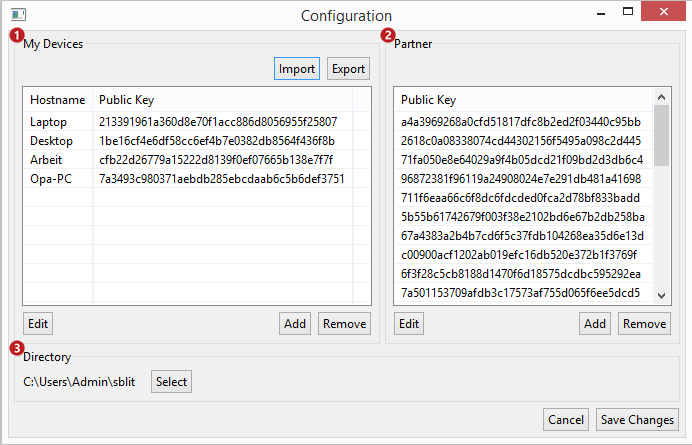
\includegraphics[]{images/config_gui.png}
	\label{ueberblicksfenster}
  \caption{Konfigurationsmenü}
\end{figure}
\begin{description}

	\item[{Geräte zu den Synchronisationspartnern hinzufügen/entfernen}]
		Unter dem Punkt “My Devices” befindet sich die Liste der
		Synchronisationsgeräte, also jene Geräte, mit denen der unter Punkt 3
		angegebene sblit-Ordner synchronisiert wird. Die Einträge
		bestehen aus dem vom Benutzer angegebenen Namen des Geräts und dessen
		Public-Key, welcher seine Adresse darstellt. Der Benutzer hat die
		Möglichkeit, bestehende Einträge für Korrekturen zu bearbeiten, neue
		hinzuzufügen oder alte zu entfernen.

	\item[{Manuelles Eintragen von Partnergeräten}]
		Obwohl die Liste der Partnergeräte automatisch von \sblit verwaltet wird,
		hat der Benutzer die Möglichkeit, Geräte manuell hinzuzufügen. Während
		nämlich normalerweise Geräte fremder Nutzer als Partnergeräte fungieren,
		kann man sich auch gegenseitig mit einer Freundin oder einem Freund
		Speicherplatz freigeben, indem man den Public-Key des jeweils anderen in der
		Liste der Partnergeräte einträgt.

	\item[{Verschieben des sblit-Ordners}]
		Der zu synchronisierende Ordner kann im Konfigurationsmenü auch nach der
		Installation noch geändert und verschoben werden.

\end{description}
